\chapter{Circuit Quantum Electrodynamics}\label{chap:cQED}
While many platforms can be used as quantum processors, our focus will be on circuits consisting of superconducting materials. In this chapter, we will go through how these qubits are designed to create qubits and how we can model these numerically. \\

\section{Circuit QED}
\begin{marginfigure}[5 cm]
    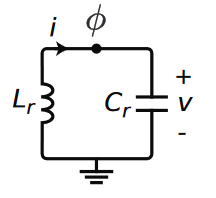
\includegraphics[width = \linewidth]{tex/fig_for_text/LC_circuit.png}
    \caption{Circuit diagram for the LC circuit.}
\end{marginfigure}
Classically\, we find the dynamics of a circuit in terms of its current $I(t)$ and its voltage drop $V(t)$. If we consider a simple circuit with one capacitor and one inductor, we have the LC circuit. To write up the energy of this system and derive the equations of motion, we consider a contribution from each of its elements. The capacitor has a charge stored in it giving an energy contribution of:
\begin{equation}
    E_{\text{capacitor}} = \frac{1}{2} CV^2 = \frac{Q^2}{2C}
\end{equation}
where $Q$ is the charge on the capacitor and $C$ is the capacitance related to the distance between two capacitance plates, the area and the permittivity of the material. We can relate the charge in the capacitor to the current by $Q(t) = Q(t_0) + \int_{t_0}^{t} dt' I(t')$. The other component is an inductor which can take many different form, one example is the coil. The inductor stores energy by having a magnetic flux through it, giving an associated energy of:
\begin{equation}
    E_{\text{inductor}} = \frac{\Phi^2}{2 L}
\end{equation}
Where $\Phi$ is the flux through the inductor and $L$ is the impendance. If the inductor was a coil, the inducatance would be related to the amount of windings, the permability materials, and its length and area. By using Faradays law, one find a relation between the current drop over the inductor and its flux: $\Phi(t) = \Phi(t_0) + \int_{t_0}^t V(t')dt'$. So if want to write the total energy (or the Hamiltonian of the system), we sum the additions from the components to give \cite{blais_circuit_2021}:
\begin{equation}
    \mathcal{H} = \frac{1}{2C} Q^2 + \frac{1}{2L} \Phi^2
\end{equation}
Which is of particular interest since $Q$ is a canonical momentum to the coordinate $\Phi$\sidenote[][-4cm]{To see this, we can rewrite the capacitor energy in terms of the flux: $\frac12 C \dot \Phi^2$ and define the lagrangian as the difference between kinetic and potential energy: $\mathcal{L} = E_{\text{capacitor}} - E_{\text{inductor}}$. Differentiating the Lagrangian with respect to the time-derivative of flux, we find $\frac{\partial}{\partial\dot{\Phi}} \mathcal{L} = Q$. \cite{krantz_quantum_2019}}. 




% The dynamics can then be calculated using the Lagrange formalism, where we find define the flux:
% \begin{equation}
%     \Phi (t) = \int_{-\infty}^t V(t')dt'
% \end{equation}
% Now using this relations together with $V = L dI/dt$ and $I = C dV/dt$ it is possible to find the energy by:
% \marginnote[0.5 cm]{The lower integration limit comes from the assumption that the system was at rest at infinity}
% \begin{equation}\label{eq: Energy from current and voltage}
%     E(t) = \int_{-\infty}^t V(t')I(t')dt'
% \end{equation}
% Such that the energy of the components are:
% \begin{equation}
%     E_{capacitor} = \frac12 C \dot{\Phi}^2; \quad E_{inductor} = \frac{1}{2L} \Phi^2
% \end{equation}
% Defining the capacitant energy as the kinetic energy $T_C$ and inductive energy as $U_L$, we can write the Lagrangian as:
% \begin{equation}
%     \mathcal{L} = T_C - U_L = \frac12 C \dot{\Phi}^2 - \frac{1}{2L} \Phi^2
% \end{equation}
% And from this the Hamiltonian:\footnote{By defining a canonical momentum $Q = \partial \mathcal{L} / \partial \dot{\Phi}$ and doing the legendre transformation $\mathcal{H} = Q\dot{\Phi} - \mathcal{L}$.} \cite{krantz_quantum_2019}:

\subsection{Going quantum}
 Usually, classical circuits exhibit energy loss due to the resistance in the material, but by creating the devices from superconducting materials and cooling them down to $\approx 30 \unit{mK}$, the superconducting phase has no resistance and will not dissipate energy\footnote{at least not through resistance. Many other outside factors can still interact with the qubit. The limited coherence is still a big obstacle for superconducting qubit.}. This allows us to quantize the variables and use the superconducting circuit as a type of artificial atom. 

Since $\Phi$ and $Q$ are conjugate variables, they satisfy the classical Poisson bracket equation:
\begin{equation}
    \{ \Phi, Q\} = \pfrac{\Phi}{\Phi}\pfrac{Q}{Q} - \pfrac{\Phi}{Q}\pfrac{Q}{\Phi} = 1
\end{equation}
To quantize these parameters, we replace the variables with the corresponding operators: $Q \to \hat{Q}$ and $\Phi \ \to \phi$. And using the correspondence principle to replace the Poisson brackets with the commutator $\{...\} \to i\hbar[...]$. Such that the quantum version of the parameters satisfy:\cite{krantz_quantum_2019}:
\begin{equation}
    [\phi, \hat{Q}] = i\hbar
\end{equation}
Since the rest of the thesis will be of quantum mechanics, we will now drop the hats from the operators and set $\hbar = 1$. We can reintroduce it later if we need to determine physical quantities. However, we will often refer to energies in terms of the associated frequency. 

\subsection{Solving the LC Circuit}\label{sec:forming_qubits}
With $Q$ and $\Phi$ conjugate variables, we can choose one to be the basis and represent the other in a differential form\footnote{Analogous to the relation between a position $x$ and momentum $p$.}.Choosing the flux basis, the charge takes the form:
\begin{equation}
    Q = i\frac{\partial}{\partial \Phi}
\end{equation}
Such that the LC circuit Hamiltonian becomes
\begin{equation}
    H \ket{\psi} = - \frac{1}{2C} \pfracsquared{}{\Phi}\ket{\psi} + \frac{1}{2L} \Phi^2 \ket{\psi}
\end{equation}
This is exactly the form of a particle in a harmonic potential and we can follow the same procedure and introduce the ladder operators$a, a^\dagger$. Such that the the Hamiltonian can be written as:
\begin{equation}
    H = \omega (a^\dagger a + \frac12)
\end{equation}
Where $\omega = \sqrt{8 E_C E_L}$ can be found by comparing the Hamiltonian with the one from the harmonic oscillator.

While the harmonic oscillator has many useful proterties, a major problem is its equidistant energy levels. When driving transitions with a pulse of frequency $\omega$, we will not only contribute drive transitions in the computational basis $\ket{0} \leftrightarrow\ket{1}$, but also to all the higher order states. This prohibits us from staying in the computational qubit space, and thus we must search for an anharmonic potential.

\section{Building Qubits}
The solution lies in another component, which is exists in the realms of superconducting circuits. By separating two superconductors by a semiconducting material, the Cooper pairs\footnote{Superconductivity is often modelled by creating electron pairs which then have spin 1 and behave like bosen. These pairs are called Cooper pairs. \cite{BCS}} will no longer travel through without resistance but will instead have to tunnel through. The probability of tunneling is dependent on the distance, material and most importantly the phase difference between the two superconductors. The probability for tunneling through the superconducting phase is given as $\sin(2e\phi(t))$, where $\phi(t)$ is the time-dependent difference in phase between the two superconductors.Using the flux-quantum $\phi_0 = h / 2e$ and adding an external flux, the current through the Josephson Junction is:
\begin{equation}
    I(t) = I_0 \sin \left( \frac{\phi(t) + \phi_{ext}}{\phi_0} \right)
\end{equation}
The energy of the Josephson Junction can now be found to\cite{krantz_week_2019}: 
\begin{equation}
    E_{\text{Josephson Junction}} = - E_J \cos \left[ \frac{\phi(t) + \phi_{ext}}{\phi_0} \right]
\end{equation}
up to a constant, which can be neglected by moving the zero point of the energy. \cite{vool_introduction_2017}

\subsection{The Cooper Pair Island}
Replacing the inductor in the LC circuit with a Josephson Junction, we get a circuit with a non-quadratic potential. The Hamiltonian is given by:
\begin{marginfigure}
    \caption{An example of a circuit with a capacitor and a Josephson Junction}
    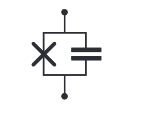
\includegraphics[width = \textwidth]{tex/fig_for_text/CooperPairIsland.png}
    \label{fig:cooper_pair_island}
\end{marginfigure}

\begin{equation}
    H(t) =  4 E_C (n - n_g)^2 -  E_J \cos \left[ \frac{\phi(t) + \phi_{ext}}{\phi_0} \right]
\end{equation}
where $n = Q/2e$ is a amount of cooper pairs on the "island" and $4E_C = 2e^2/C$, where the factor of 4 would disappear if we counted electrons instead of pairs. Like flux and charge, the Cooper Pair number $n$ and the superconducting phase difference $\phi$ form a canonical commutation pair: $\comm{n}{\phi} = i$. In In the Cooper Pair Box the energy scales of the two contributions are approximately equal $E_C \approx E_L$ \cite{blais_circuit_2021}. 


\begin{figure}
    \centering
    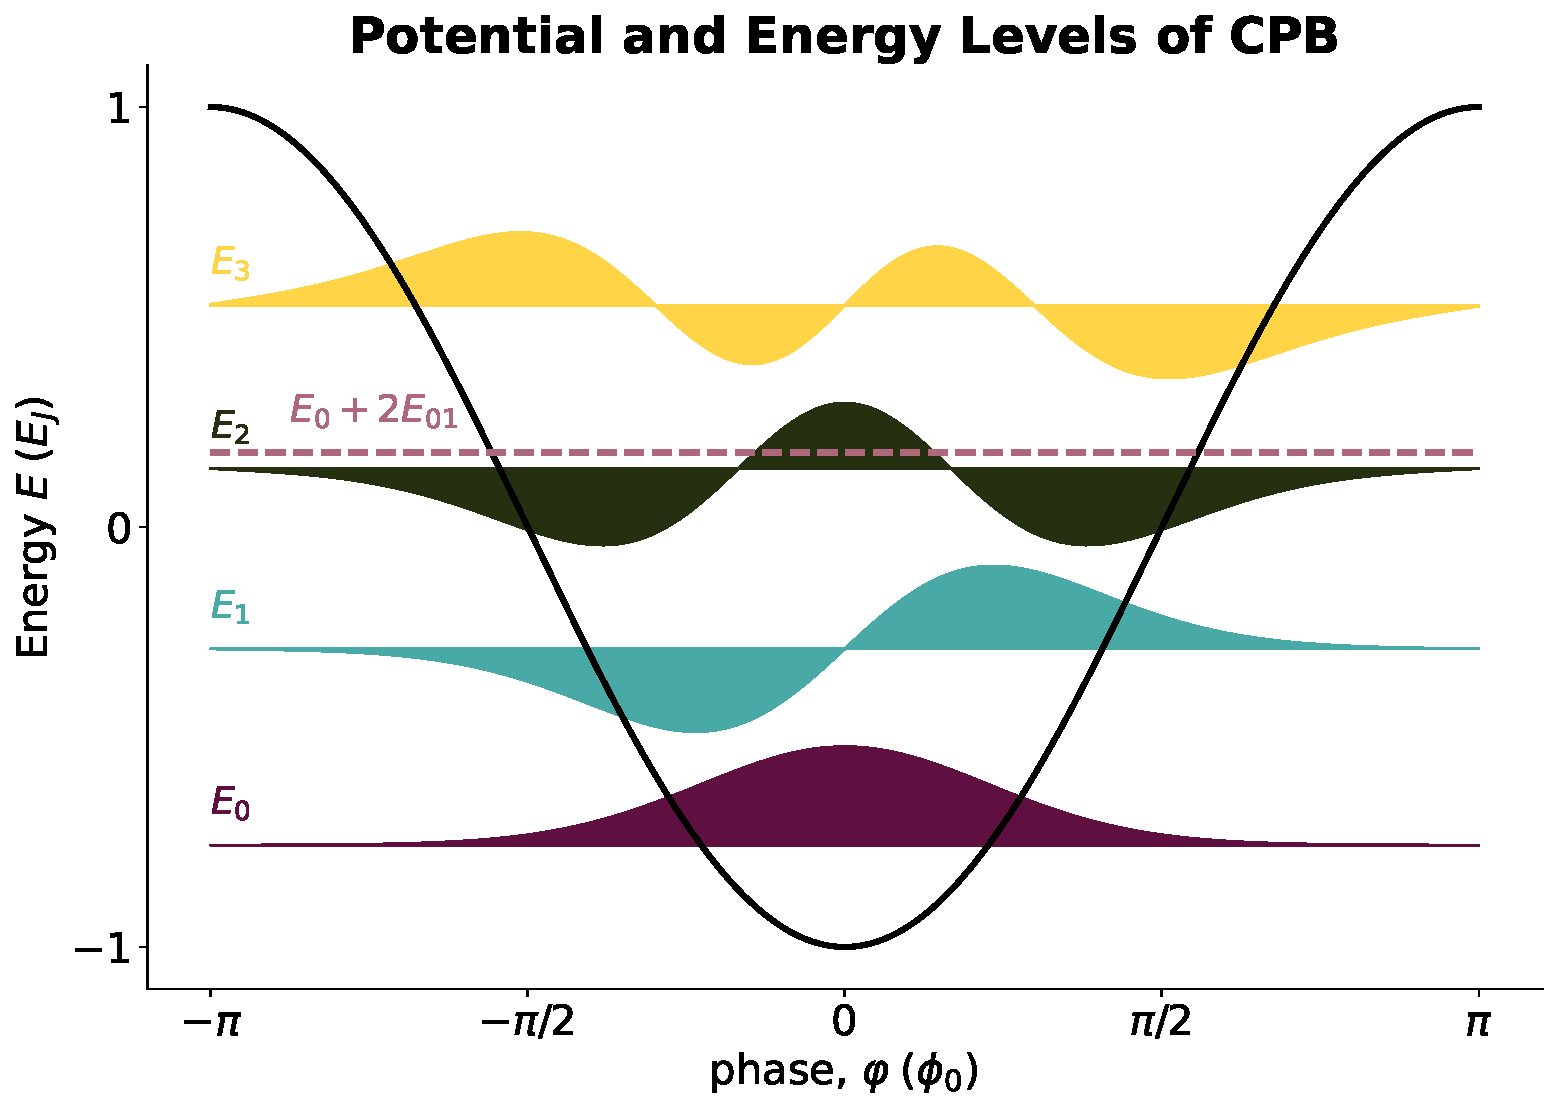
\includegraphics[width=1.00\linewidth]{Figs/Theory/CPB_potential.pdf}
    \caption{The flux-potential of the cooper pair box along with the three lowest energy eigenstates. The eigenstates are shifted according to the theiry energy and scaled to improve readability. The energy level $E_0 + 2E_{01}$ is shown for comparison. The anharmonicity will be the difference between that line and the $E_2$}
    \label{fig:cooper_pair_box_energy_levels}
\end{figure}


This allows us to think about $\phi$ as a coordinate where the Josephson Junction energy defines a potential and the charge a kinetic energy. Solving the eigenvaue problem $H\psi(\phi) = E \psi(\phi)$, we can find the eigenenergies and the eigenvectors of the Cooper Pair Island in $\phi$-space. A solution to this problem with $E_C = E_L$ can be seen in figure \ref{fig:cooper_pair_box_energy_levels}. Most importantly, we note that the that the energy $E_2-E_1 \neq E_1 - E_0$. This difference is called \textit{anharmonicity} and is defined by $\alpha = (E_2 - E_1) - (E_1 - E_2)$ \cite{krantz_week_2019}.

\subsection{The Transmon}
With $E_J / E_C \approx 1$ the circuit is susceptible to noise in the charge. Since charge noise is harder to control than flux noise, the superconducting community has moved toward higher ratios for $E_J / E_C$. Most commonly the fraction is somewhere between 50 and 100. As can be seen in figure \ref{fig:transmon_charge_sensitivity} the energy of the states is not a sensitive to changes in the charge. Like most design choices this does not come for free and the cost here is  anharmonicity. With lower anharmonicity, we need longer pulses to make sure, we do not accidental have components of the $E_2 - E_1$ frequency in our pulse \cite{koch_charge_2007}. 
\begin{figure}
    \centering
    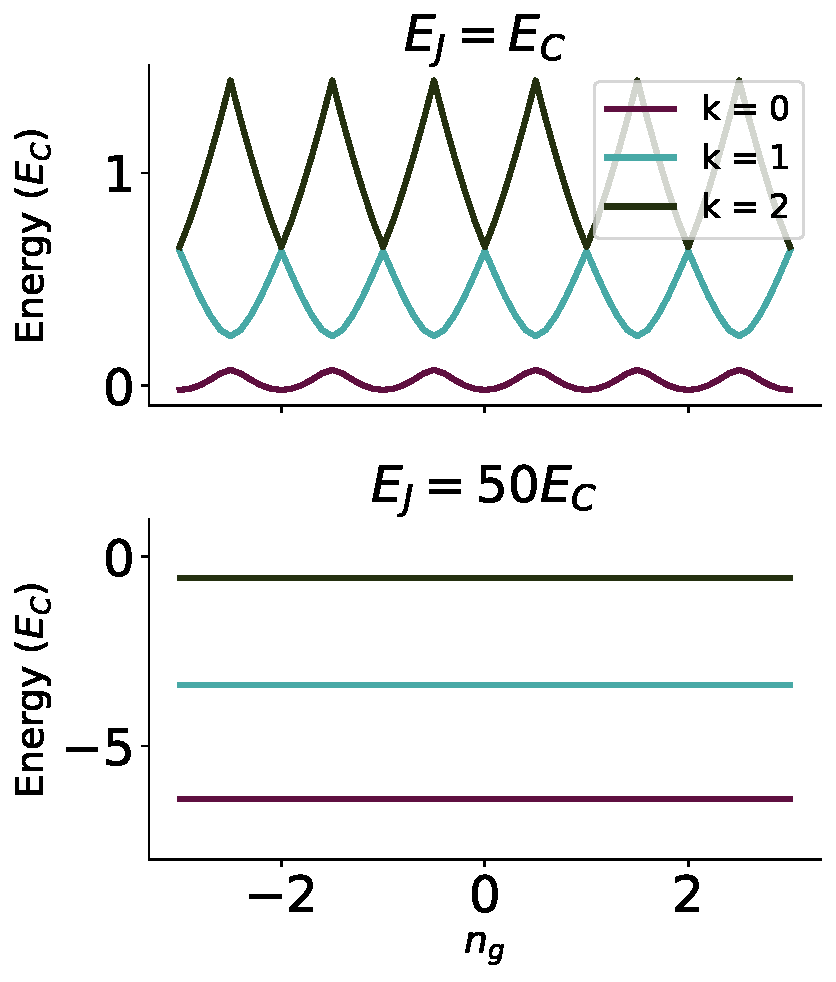
\includegraphics[]{Figs/Theory/Transmon_energy_vs_ng.pdf}
    \caption{The energy levels of the Transmon at different levels of $E_J / E_C$.}
    \label{fig:transmon_charge_sensitivity}
\end{figure}
Multiple additions can be made to the Transmon to make its energy tuneable. Two possibilities are to either replace one Josephson Junction with two in a loop. This creates a SQUID and by adjusting the flux through it the energy can be tuned \cite{blais_circuit_2021}. 



\section{Numerical cQED}
In an attempt to simulate the systems considered in this thesis, we will in this section introduce how the problems at hand is represented in a suitable way for solving numerically. As mentioned in the previous sections, the Hamiltonian is made out of the two conjugate operators $\phi$ and $n$ satisfying the commutation relation $\comm{\phi}{n} = i$. Like the position and momentum, we now have a choice of which basis to represent the system in. In mechanical quantum problem, we would for example consider the position basis ${x}$ and the momentum $p$. These two basis are related by Fourier transformations, and we get\footnote{This is very similar to the relation between $x$ and $p$, but with the extra detail that $n$ is discrete and $\phi\in[0, 2\pi]$}  \cite{langford_circuit_2013}:
\begin{align}
    \ket{\phi} &= \sum_{n=-\infty}^\infty e^{in\phi}\ket{n} \\
    \ket{n} &= \frac{1}{2\pi} \int_0^{2\pi}d\phi e^{-in\phi}\ket{\phi}
\end{align}
Often the problem at hand is easier to formulate in one basis rather than the other. For the transmon, the charge is often localized around 0 since higher $n- n_g$ values give very high energies. This will allow us to set a limit on the $n_{\text{cutoff}}$ and is probably a good choice for formulating the numerical problem. In the charge basis, the energy associated with $\hat{q} = 2e\hat{n}$ takes a diagonal form which at finite dimensions can be represented as:

\begin{fullwidth}
\begin{equation}
    \hat{q} =  2 e \hat{n} = 2 e \begin{pmatrix}
-n_{\text{cutoff}} & 0 &  & \ldots &  \\
0 & -n_{\text{cutoff}}+1 &  &  &  \\
 &  & \ddots &  &  \\
\vdots &  &  & n_{\text{cutoff}}-1 &  \\
 &  &  &  & n_{\text{cutoff}} 
\end{pmatrix}
\end{equation} 
\end{fullwidth}

To represent the full Hamiltonian we now need $\cos(\phi / \phi_0)$ in the charge basis. Here we will use that:
\begin{align*}
    e^{\pm i \phi}\ket{n} &= \frac{1}{2\pi} \int_0^{2\pi} d \phi' e^{-in\phi'} e^{\pm i \phi}\ket{\phi'} \\
                                &=  \frac{1}{2\pi} \int_0^{2\pi} d \phi' e^{-in\phi'\pm i \phi'} \ket{\phi'} \\
                                &=  \frac{1}{2\pi} \int_0^{2\pi} d \phi' e^{-i\phi'(n\pm 1)} \ket{\phi'} = \ket{n\mp 1}\\                                
\end{align*}
Since it is true for all states that the operator $e^{i\phi}$ takes a state $\ket{n}$ to $\ket{n+1}$, we can write it in charge basis as:
\begin{equation}
    e^{i\phi} = \sum_n \ket{n}\bra{n+1}; \quad e^{-i\phi} = \sum_n  \ket{n}\bra{n-1}
\end{equation}
Just rewriting cosine in terms of the Euler into complex exponentials, we find 
\begin{fullwidth}
\begin{align}
    \cos(\phi/\phi_0 + \phi_{ext}) &= \frac12 \left(e^{-i(\phi/\phi_0 + \phi_{ext})} + e^{i(\phi/\phi_0 + \phi_{ext}}))\right) \\
    &= \frac12 \left(e^{i\phi_{ext}}e^{i\phi/\phi_0} + e^{-i\phi_{ext}}e^{-i\phi/\phi_0}\right)  \\
    &= \frac12 \sum_n \left(e^{i\phi_{ext}} \ket{n}\bra{n + 1} + e^{-i\phi_{ext}} \ket{n}\bra{n+ 1}   \right) \\
    &= \frac12 \begin{pmatrix}
        0 & e^{-i\phi_{ext}} & 0 & \hdots \\
        e^{i\phi_{ext}} & 0 & e^{-i\phi_{ext}} \\
        0 & e^{i\phi_{ext}} & 0 & \\
        \vdots & & & \ddots 
    \end{pmatrix}
\end{align}
\end{fullwidth}
If we consider no external flux, $\phi_{ext} = 0$, then cosine is a matrix with elements equal to $\frac12$ on the off-diagonals. 

If a problem instead would have been more convenient in the flux basis, we could have started with matrix with the diagonal representation of flux, where the diagonal is $(-\pi, -\pi + \delta \dots, \pi)$. Here $n$ would take a discrete form of the differential $i\pfrac{}{\phi} \approx \frac{i}{2\delta} \sum_k (\ket{-\pi + k\delta}\bra{\pi} + \ket{\pi}\bra{-\pi + k\delta})$ \cite{aumann_circuitq_2022}.

With a discrete matrix representation of the charge matrix and flux operators, we are in a position to calculate the eigenenergies and states of a given Hamiltonian. This is done by numerically determining the eigenvalues/vectors of the Hamiltonian matrix. By limiting us to the few lowest energy eigenstates because of the low temperature, we can reduce the basis significantly to the energy representation, where the Hamiltonian is diagonal: $H = \sum_k^{k_{max}} \hbar \omega_k \ket{k}\bra{k}$ where $k$ refers to the k'th lowest energy eigenvalue of the Hamiltonian. We can then further find the charge matrix as $\mel{k}{q}{k}$ and so forth. \todo{What is a good figure here?}


% \textbf{Rambling now. Tighten the following: from . The part with }

% When considering the circuits like the transmon with $\frac{E_C}{E_J}\approx 50$ the dominating term in the hamiltnonian will be the contribution from the charge offset proportional to $(\hat{n} - n_g)^2$. This is a good indication that the charge matrix would be good choice to contain as much information as possible near the diagonal. In the charge basis the charge matrix simply takes the form:

% where $n_{\text{cutoff}}$ is an appropriately set parameter to limit the size of our hilbert space. With the parameters used, this is normally set around 50-100. \\

% With the choice of $n$ as eigenbasis the operator representation for flux will be $\phi = \pfrac{}{\hat{n}}$ in the continuous basis or for finite dimensional Hilbert space, we have:
% \begin{equation}
%     \phi = 
% \end{equation}

% \textbf{Probably do the transmon in the flux basis? }





% \vspace{2 cm}
% \textbf{This could also be a numerical section between section 2.1 and 2.2 which we can base the cooper pair box on. }
% When using the transmon, we use the energy eigenstates as a computational basis. To figure out, how the energy splitting and reactions to charge are, we need to find these energy eigenenergies and states.

% \begin{itemize}
%     \item Start with charge basis
%     \item We can now represent the flux as a potential
%     \item Solving numerically gives lowest eigenenergy and states
%     \item Calculating certain matrix elements between the eigenstates givers us the charge-matrix, flux-matrix, etc.. 
% \end{itemize}


\section{Experimental Setup}
While most of the work in this thesis will be theoretical and computational, we will try to understand, calibrate and model a physical system. This section will serve as a short introduction.
\todo{Write this section properly.}

\subsection{Soprano Chip}
The experiments are run on the Soprano 6 qubit Chip on qubit ? (see figure \ref{fig:soprano}), a flux tuneable transmon connected to a resonator, drive line and flux line to tune the transmon. The resonator is connected to a feed line which is further connected to the five other resonators (some through a purcell filter).

\begin{figure}[h]
    \begin{minipage}{0.50\textwidth}
        \centering
        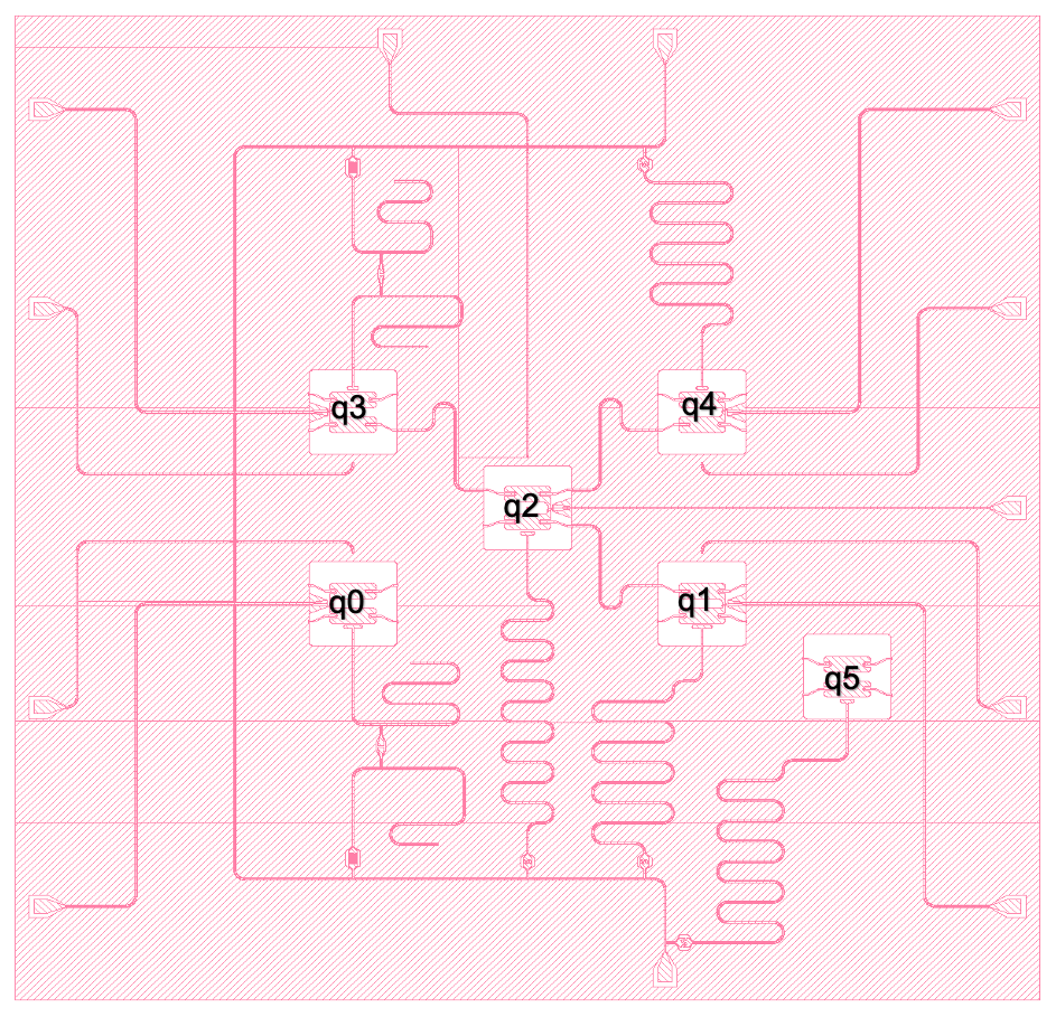
\includegraphics[height = 5 cm]{Figs/hardware/layout.png}
    \end{minipage}
        \begin{minipage}{0.50\textwidth}
        \centering
        \includegraphics[height = 5 cm]{Figs/hardware/layout_photo.png}
    \end{minipage}
    \caption{The Soprano Chip layout and a picture.}
    \label{fig:soprano}
\end{figure}

\subsection{Cooling and Amplification}
To keep the soprano chip cold, it is places in a Cryostate capable of cooling to $\approx 30 \text{mK}$ while keeping the chip in vaccum to reduce thermal fluctuations and interactions with the environment. 

\begin{itemize}
    \item Down Conversion Line
    \item Up Conversion Line -> TWPA -> higher temperature amplifiers 
\end{itemize}


\subsection{Control Hardware}
At room temperature the microwave pulses are generated by an Arbitary Waveform Generator in the form of an OPX. The signal from the OPX enters an Octave where it is mixed by an internal local oscillator to convert the microwaves from $\approx 500 \text{ MHz}$ to the suitable $5$ to $10 \text{ GHz}$ before interacting with the qubit or resonator. 

In the down-conversion line, the readout signal from the cryostate enters the octave, where it enters and IQ mixer splitting the signal in two. After mixing with the local oscillator again it is send back to OPX where it enters a digital to analogue converter before being demodulated and integrated.





